\documentclass{article}
\usepackage[german]{babel}
\usepackage[utf8]{inputenc}
\usepackage{tabularx}
\usepackage{listings}
\usepackage{graphicx}
\usepackage{float}
\usepackage{url}
\newenvironment{funcD}{\vspace{-.6cm}\\\par\begingroup\leftskip=.4cm\noindent\\}{\\\par\endgroup\noindent}

\usepackage[
  style=alphabetic, % Loads the bibliography and the citation style
  % bibstyle=alphabetic, % load a bibliography style
  % citestyle=alphabetic, % load a citatio style
  natbib=true, % define natbib compatible cite commands
%%--- Backend --- --- ---
  backend=biber,   % (bibtex, biber)
  bibwarn=true,     %
  texencoding=auto, % auto-detect the input encoding
  bibencoding=auto, % (auto (equal to tex), <encoding>)
]{biblatex}
\addbibresource{references.bib}

\title{Projektbericht TranscriptionDesk}
\author{Robert Rößling, Jakob Runge, Oliver Schurig, Franz Teichmann}
%\date{März 2015}

\begin{document}
%TODO: Stets zwei-drei Sätze Kapiteleinleitung beachten, englische Fachbegriffe auf ein Minimum reduzieren und nicht mehrere Begriffe für eine Semantik nutzen
% z.B. Nutzer statt User, Projekt statt Praktikum
%TODO genaue Beschreibung des Projektes erfolgt erst nach der analyse und Einordnung

\maketitle

\subsection*{Abstract}
Das TranscriptionDesk Projekt umfasste Konzeption und Entwicklung einer webbasierten Plattform,
auf der sich unterschiedlich versierte Nutzer zwecks Mitarbeit an der Transkription
einer großen Datenbasis aus Scans mittelalterlicher Handschriften registrieren können.
Dies beinhaltet außerdem die Analyse der Scans in Bezug auf die Unterscheidung zwischen Originaltext und nachträglicher Annotation.
Alle Quelldateien mit Dokumentation, Installationsanleitung und diesem Projektbericht
stehen unter MIT Lizenz und sind digital veröffentlicht unter \url{https://github.com/runjak/TranscriptionDesk}.

\tableofcontents
\newpage

\section{Einleitung}
Das Projekt TranscriptionDesk wurde im Zuge des Moduls ,,Citizen Science'' an der Universität Leipzig im Sommerstemester 2015 durchgeführt.
Das Thema umfasste die Konzeption und Entwicklung einer Webplattform nach dem Paradigma der Citizen Science,
welche eine dynamische Transkription einer großen Datenbasis bestehend aus Scans mittelalterlicher Handschriften ermöglicht.
In dieser Arbeit sollen die Hintergründe sowie unsere Ideen und Gedankengänge auf dem Weg vom Thema zum konkreten Projektauftrag,
die von uns betrachteten (Teil-)Aufgaben sowie die Ergebnisse präsentiert
und die Architektur der entstandenen Software beschrieben werden.
Dazu sollen zunächst die theoretischen Grundlagen erläutert werden,
um daraus im Anschluss unsere Projektdefinition abzuleiten und
die Überlegungen aus der Planungsphase zusammenzufassen.
Danach soll ein direkter Einstieg ins Projekt mit der Darstellung der Architektur und der Produktfunktionen erfolgen und auf Funktionen hingewiesen werden,
welche bisher aufgrund des begrenzten Zeitrahmens nicht umgesetzt werden konnten.
Am Schluss des Berichtes wird eine Zusammenfassung der ,,lessons learned'' sowie ein Ausblick auf mögliche Folgeprojekte gegeben.

\section{Theoretische Grundlagen}
In diesem Kapitel sollen die Grundlagen für die späteren Erläuterungen gelegt werden.
Dazu soll zunächst die Definition von Citizen Science aus der Vorlesung rekapituliert und auf verschiedene Deutungen des Begriffes eingegangen werden, um anschließend eine Arbeitsdefinition als Plan für unser Projekt abzuleiten und diesen in die Kategorien der Citizen Science nach Crowston und Wiggins einzuordnen.
Es sei hierbei auch auf Literatur zum Thema verwiesen.

Es handelt sich bei ,,Citizen Science'' um einen verhältnismäßig neumodischen Begriff
für ein gleichnamiges Teilgebiet der angewandten Sozial- und Geisteswissenschaften,
was nicht bedeutet, dass die Idee hinter dem Begriff Citizen Science grundsätzlich neu ist.
Tatsächlich lassen sich Aktivitäten, die heutzutage unter diesem Begriff zusammengefasst werden,
fast 200 Jahre in der Geschichte zurückverfolgen.
Anwendungsmöglichkeiten und die Komplexität dieses Themengebietes
wurden uns im Laufe der Lehrveranstaltung an aktuellen sowie an historischen Beispielen veranschaulicht
und sowohl Gemeinsamkeiten als auch Unterschiede zwischen den verschiedenen in den Beispielen verfolgten Ansätzen herausgearbeitet.
Da es keine ,,einfache'' oder ,,schnelle'' Definition gibt, die diesen Sachverhalt vollständig beschreibt,
versuchen wir die Komplexität noch einmal in den zwei folgenden Unterkapiteln einzufangen
und einer Definition so nahe zu kommen, wie es uns möglich ist.

\subsection{Definition Citizen Science}
Der Frage nach der Definition von Citizen Science versucht Wiederhold\cite{Wiederhold} (S.703-4) in ihren Arbeiten mit der Annäherung über den Begriff des ,,Citizen Scientist'' zu beantworten.
Es werden dazu aktuelle Entwicklungen, wie etwa das relativ bekannte FoldIt-Spiel\footnote{
FoldIt ist ein Onlinespiel, das sich mit Eigenschaften von Proteinen befasst. Der Spieler benötigt keinerlei biologisches Hintergrundwissen,
sondern ein Gefühl für räumliche Bewegung der Spielelemente.
Spielergebnisse liefern wertvolle Daten für Wissenschaftler und haben zu wichtigen Erkenntnissen in der Virenforschung geführt. \url{https://fold.it/portal/}},
sowie historische Beispiele betrachtet, die in die Citizen Science eingeordnet werden.
Eines der ältesten bekannten Projekte, so Wiederhold, ist das National Audubon Society's Christmas Bird Count-Projekt\footnote{Das Projekt wurde 1900 von Frank M. Chapman gegründet.
Ziel war es, Vogelarten zu bestimmen und zu zählen, um der bis dahin üblichen ,,Side Hunt'',
die jedes Jahr zur Weihnachtszeit Jäger dazu herausforderte, so viele Vögel wie möglich zu schießen,
eine umweltverträgliche Alternative zu bieten. \url{https://www.audubon.org/conservation/science/christmas-bird-count}}.
Auch heute ist dieses Projekt noch relevant, wie die dazu existierende Homepage mit aktuellen Nachrichten verdeutlicht.\\
Diese zwei Beispiele lassen gleichzeitig auch eine Bereicherung der historischen Citizen Science durch die digitale Welt erkennen.
Obwohl viele bekannte Projekte weiterhin unter ,,Environmental Science'', wie Wiederhold sie nennt, einzuordnen sind,
besteht in einer großen Anzahl der Projekte die Arbeit für den Citizen Scientist nur aus nicht maschinell abstrahierbarer Computerarbeit,
welche wenig bis keine Vorkenntnisse erfordert.\\
Unter Berücksichtigung dieser Betrachtungen definiert Wiederhold den Citizen Scientist nach Cohn\cite{Cohn}:
,,The term 'citizen scientists' refers to volunteers who participate as field assistants in scientific studies.
Citizen scientists...are not paid for their assistance, nor are they necessarily even scientists.''(58:192-7).
Diese Definition beschreibt treffend die Rahmenbedingungen, unter denen ein solcher Citizen Scientist arbeitet
und in welche Themengebiete er sich einbringt, jedoch lässt sie entscheidende Aspekte für die Definition der Citizen Science selbst vermissen.\\
Fragen die nicht beantwortet werden, sind beispielsweise solche nach dem Rahmen bei der Bestimmung einer Forschungsfrage,
dem notwendigen Grad an Wissenschaftlichkeit des Projektes, oder auch welche Finanzierungsmöglichkeiten für derartige Projekte bestehen.
Der Idee der Definition über den Citizen Scientist folgend beschreibt Cohn Citizen Science als
,,die wissenschaftlichen Aktivitäten in denen nicht-professionelle Wissenschaftler sich freiwillig an Datensammlung,
Analyse und Verbreitung eines wissenschaftlichen Projekts beteiligen.''\cite{Cohn}.\\
Für ihn ist der Citizen Scientist eindeutig wissenschaftlich tätig und dieser Aspekt spielt eine entscheidende Rolle
bei der Konzeption von Projekten. Unserer Meinung nach ist diese Definition treffend und für unser Projekt präzise genug,
auch wenn die Frage nach den Finanzierungsmöglichkeiten vorerst unbeantwortet bleibt.\\
Auch wird in dieser Definition keine klare Grenze zum Crowdsourcing
\footnote{Crowdsourcing: Bezeichnend für das Auslagern interner Aufgaben eines Unternehmens an Freiwillige Nicht-Angestellte.
Angelehnt an den Begriff Outsourcing, bei dem Drittunternehmen ausgelagerte Aufgaben verrichten.
Häufig wird Crowdsourcing über das Internet realisiert.} gezogen.\\
Um diese Fragen für uns beantworten zu können, befassten wir uns mit unterschiedlichen, bereits existierenden Projekten.
Einige davon gehörten eindeutig zum Crowdsourcing, andere wiederum waren für uns nicht so eindeutig zuzuordnen.
Gewissermaßen kann man also Crowdsourcing und reine Citizen Science als zwei gegensätzliche Pole einer Skala betrachten.
Dieser Meinung ist auch Haklay\cite{Haklay} (pp 105-122), der eine solche Skala näher analysierte,
worauf im kommenden Kapitel eingegangen werden soll.
Auch Crowston und Wiggins\cite{CW} leisteten bedeutende Arbeit für die praktische Einordnung von Projekten in die Citizen Science.
Laut ihren Untersuchungen lässt sich das Spektrum der Projekte in folgende fünf Kategorien unterteilen:
,,Based on the clustering, we identified five mutually exclusive and exhaustive types of projects,
which we labelled Action, Conservation, Investigation, Virtual and Education'' (S. 5).
Auch diese sollen im Folgekapitel noch einmal einzeln Erwähnung finden.


\subsection{Kategorien der Citizen Science}

Nach Hacklay existieren folgende vier Abstufungen\cite{Haklay} (pp 115) in der Charakterisierung von Projekten zwischen Citizen Science und Crowdsourcing.
\begin{enumerate}
\item{Level 1: Crowdsourcing\\
Hier hat die einfache Nutzerschaft lediglich die Aufgabe der Datenerhebung, die Interpretation erfolgt an anderer Stelle.}
\item{Level 2: Distributed Intelligence\\
Auf diesem Level sollen freiwillige Nutzer Denkarbeit verrichten und werden dabei grundlegend für interpretative Aufgaben eingesetzt.}
\item{Level 3: Participatory Science\\
In dieser Kategorie werden die Freiwilligen bereits in der Problemdefinition mit einbezogen, sie übernehmen aber auch Aufgaben zur Sammlung von Daten.}
\item{Level 4: Extreme Citizen Science\\
Diese Kategorie betrachtet den gesamten wissenschaftlichen Prozess als kollaborative Aufgabe für die freiwillige Nutzerschaft.
Sie nimmt an der Problemdefinition ebenso teil wie an der Sammlung von Daten und deren Analyse.}
\end{enumerate}
Während Haklay versucht, den Unterschied der Citizen Science nach außen abzugrenzen, gibt es wie im letzten Kapitel beschrieben auch
Bestrebungen, die Citizen Science in aussagekräftige Kategorien zu teilen. Crowston und Wiggins definierten hierfür folgende fünf Cluster:
\begin{itemize}
\item{Action\\
Bei Action handelt es sich um Projekte, die ihren Ursprung häufig in einem lokal begrenzten Umfeld haben.
Sie werden nicht durch Wissenschaftler in die Wege geleitet,
sondern durch ,,einfache'' Leute, die einen singulären Handlungsbedarf sehen und eine Bewegung für Freiwillige ins Leben rufen.
Für gewöhnlich geht es dabei um Ziele, welche die Umwelt betreffen.
Technologien kommen dabei nur minimal zum Einsatz, soweit sie von Notwendigkeit sind.}
\item{Conservation\\
Conservation befasst sich mit dem Management und Erhalt der natürlichen Ressourcen bzw. Biodiversität.
Freiwillige haben dabei häufig Verwaltungsaufgaben oder sind dafür zuständig, eine breitere Masse zu erreichen.
Folglich ist auch Wissensvermittlung ein untergeordnetes Ziel, dieser Art von Projekten.
Finanzierung ist oft ein Problem, das nur über staatliche Gelder gelöst werden kann und oft
zu starker Abhängigkeit von entsprechenden Stellen führt.}
\item{Investigation\\
Investigation hat wissenschaftliche Datenerhebungen zum Ziel.
Hier werden Daten von Freiwilligen im physikalischen Umfeld gesammelt.
Bildung und Wissensvermittlung sind hier zwar kein explizites Ziel, oft jedoch sind Vorkenntnisse der freiwilligen Helfer ein Faktor,
der die Arbeit erheblich genauer und effizienter gestaltet.}
\item{Virtual\\
Virtual weist viele Parallelen zu Investigation auf, spielt sich jedoch in virtueller Umgebung ab.
Besonders hier ist es nicht so leicht, die Teilnehmer als Citizen Scientists wahrzunehmen, da sie oft nur eine Zwischeninstanz darstellen,
welche Daten verarbeitet.
Probleme, mit denen man sich hier besonders befassen muss sind die Validierung der Daten und das Management
einer große Masse an Nutzern, die auf teilweise sehr komplexen Plattformen agiert.}
\item{Education\\
Education hat, wie der Name vermuten lässt, einen primären Bildungsauftrag.
Nicht immer ist es dabei leicht, ausreichend Gelder über Sponsoren zu erhalten, da meist nur ein geringer wissenschaftlicher oder
wirtschaftlicher Mehrwert erzielt wird.}
\end{itemize}
Sicher lassen sich noch wesentlich mehr Kategorien für konkrete Anwendungsfälle finden,
doch für den Zweck der Charakterisierung und Einordnung unseres Projektes sollen die Arbeiten von Haklay sowie Crowston und Wiggins
als Referenzen genügen.

\subsection{Einordnung des TranscriptionDesk}
Unserer Einschätzung nach ist TranscriptionDesk aufgrund der Aufgabenstellung der interpretierenden Transkription auf Haklays Skala näher am
Crowdsourcing als an der extreme Citizen Science einzuordnen.
Das Level 2, also die ,,Distributed Intelligence'' erscheint uns passend, da die freiwilligen Mitarbeiter eine Analyse, also eine klare Denkleistung durchführen sollen.
Außerdem ist mit der Problemdefinition das Projektziel bereits vorgegeben, so dass die Vorraussetzungen für Level 3 nicht gegeben sind.\\
Schauen wir uns die Kategorien von Crowston und Wiggins an, so müssen wir TranscriptionDesk zwangsläufig zur Kategorie ,,Virtual'' zählen.
Alle Faktoren des Projektes treffen exakt zu.\\
Auch einige wenige Faktoren der Action-Kategorie werden ebenfalls erfüllt, da Beispielsweise der Ursprung des Projektes darin liegt,
dass Daten vorhanden sind, die transkribiert und validiert werden müssen und somit eine Notwendigkeit zum Handeln den Ausschlag für das Projekt gab.
Das Hauptargument gegen die Action-Kategorie ist, dass es keine lokal begrenzten, umweltbezogenen Faktoren für den Handlungsbedarf gibt.

\section{Projektübersicht}
In diesem Kapitel soll mit einer detaillierten Übersicht über das Projekt und dessen Zielstellung ein direkter Einstieg geben werden.
Dazu soll ausgehend von der Projektvision die Struktur der Datenbasis erläutert und die erwartete Nutzerbasis reflektiert werden.

\subsection{Ziele}
Unser Projektthema fand seine Motivation in der Abteilung der Digitalen Geistes-wissenschaften der Universität Leipzig.
Dort liegen tausende Scans mittelalter-licher Schriftstücke vor, deren Informationsgehalt ohne vorherige Transkription nicht digital zu verarbeiten ist.
Es wurde als unmöglich bewertet, den Inhalt der Schriftstücke mittels typischer Optical-Character-Recognition-Methoden (OCR) sinnvoll zu digitalisieren.
Das hat im Wesentlichen zwei Gründe.\\
Einerseits war Papier im Mittelalter Mangelware und somit ein wertvolles Gut, welches sparsam verwendet wurde.
Deswegen nutzte man freien Platz gut aus und es gibt Passagen,
die nicht in einen gemeinsamen zeitlichen Kontext gehören (z.B. nachträgliche Annotationen) und somit händisch getrennt werden müssen.
Der Fakt, dass die Schriftstücke aufgrund ihres Alters bereits durch viele Hände gegangen sind und im Laufe der Zeit
mit unterschiedlichen Handschriften auf dem Papier gearbeitet wurde, erschwert OCR umso mehr.
Diese Informationen sollen entsprechend getrennt und digitalisiert werden.\\
Der zweite Grund besteht darin, dass das Schriftbild des Mittelalters oft künst-lerisch aufgewertet wurde.
So waren Texte in Blockform sehr beliebt und man erfand allerlei unterschiedliche Formen für semantisch gleichbedeutende Buchstaben,
die durch ihre Vielfalt für einen OCR-Algorithmus praktisch unmöglich zu lesen sind.\\
Die Aufgabe, welche sich daraus ergibt, kann praktisch nur durch akribische, händische Arbeit gelöst werden.
An dieser Stelle soll die Citizen Science ins Spiel kommen; durch den Aufbau einer Webplattform könnte ein großer Teil der Arbeit nach außen,
an Freiwillige mit unterschiedlichen Erfahrungen und unterschiedlichem Wissen abgegeben werden.
Dadurch soll die Digitalisierung der auf den Scans enthaltenen Texte beschleunigt, wenn nicht erst ermöglicht werden.\\
Das Ziel, das wir vor Augen haben ist also der Aufbau einer Weboberfläche, welche die Scans einer offene Gruppe freiwilliger Nutzer anbietet,
ihnen die Werkzeuge für deren Bearbeitung bereitstellt, die Ergebnisse speichert, und der Nutzerschaft die Möglichkeit bietet,
ihre gegenseitigen Ergebnisse zu bewerten, um ein einheitliches Level an Validierung der digialisierten Texte anzustreben.
Die Seite soll so strukturiert sein, dass sie weitestgehend selbstverwaltend ist und lediglich einige wenige Administratoren
die verbleibenden Verwaltungsaufgaben erledigen können.
Dabei ist auch die Möglichkeit gegeben, diese Administratoren ebenfalls in Teilen aus der Nutzerbasis zu beziehen.\\
Die Arbeit für einen Nutzer soll aus zwei unterschiedlichen Aufgaben bestehen.
\begin{itemize}
\item{Erstere besteht darin, Rechtecke auf den Scans zu ziehen, um ,,Areas of Interest'' zu markieren.
Dies können beispielsweise Bilder oder zusammengehörende Textfetzen sein.
Das Ergebnis ist eine Interest Map eines Scans, die andere Nutzer bewerten können, um deren Akzeptanz wiederzuspiegeln.
Scans können direkt ausgewählt oder per Zufall zugeordnet werden.}
\item{Die zweite Aufgabe besteht aus der eigentlichen Transkription.
Eine Interest Map wird verwendet und die darauf enthaltenen Areas of Interest werden vom Nutzer mit einer Transkription versehen.
Auch dieses Ergebnis wird gespeichert und bewertet und es wird ein bestes Ergebnis ermittelbar.}
\end{itemize}
Unsere Aufgabe ist es dabei, all diese Funktionen als Grundfunktionalität zu implementieren und sie ansprechend zu gestalten.
Der letzte Punkt ist für uns sehr wesentlich, da bei unserer Recherche auffiel, dass ähnliche (und darunter technisch gesehen sehr gute)
Projekte bereits an kleinen Schönheitsfehlern scheitern mussten, weil die Nutzer sich einfach nicht angesprochen fühlten.
Zusätzlich gehört es aus mehreren Gründen zu unserem Ziel, eine Login-Routine für das User-Management aufzubauen.
Dies bietet viele Vorteile beim Verfolgen von Veränderungen, für eine faire Verteilung von Bewertungen,
oder etwa um Statistiken einzelner oder auch aller Nutzer zu erstellen.\\
Außerdem besteht eine unserer wichtigsten Aufgaben darin, auf der gesamten Weboberfläche Unicode verwendbar und lesbar zu machen.
Ganz speziell bedeutet das, das wir eine sehr umfangreiche Eingabemaske aufbauen müssen,
die einen mächtigen Satz an mittelalterlichen Sonderzeichen in einer nutzerfreundlichen Art und Weise hergibt.
Die Identifikation von Scans erfolgt über Cite URNs\footnote{\url{http://www.homermultitext.org/hmt-doc/cite/cite-urn-overview.html}}.
Wir wollen die Areas of Interest durch Erweiterung des Konzeptes ebenfalls über jene Cite URN identifizieren können.\\
Die bisher genannten Features haben die höchste Priorität und bilden die Grundfunktionalität unserer Weboberfläche.
Ab diesem Punkt lassen sich schrittweise weitere Features hinzufügen um die Arbeit zu erleichtern, angenehmer oder einfach ansprechender zu gestalten.
Deswegen haben wir unsere anfängliche Planung mittels Scrum an ein agiles Entwicklungsmodell angelehnt.\\
Zuerst planten wir unsere grobe Architektur sowie diverse Technologien, die wir verwenden könnten.
Auf beides werden wir in Folgekapiteln noch einen genaueren Blick werfen. Dann wurden drei Meilensteine geplant,
wobei der erste davon für die Erstellung der Nutzerauthentifikationsroutine und die Anbindung der im Hintergrund genutzten Dienste enthielt.
Im zweiten Meilenstein ging es im Prinzip um alles, was die Maske der Weboberfläche sowie die Implementation der Arbeitswerkzeuge für die Nutzer betrifft.
Damit sollte die Grundfunktionalität weitestgehend aufgebaut sein. Für alle Eventualitäten soll es noch einen dritten Meilenstein geben,
in dem konkrete Bugs gelöst werden sollen und, falls dann noch ausreichend Zeit bleibt, direkt weitere Funktionen implementiert werden können.
\subsection{Struktur der Datenbasis}
Die Scans, die den Bedarf nach der TranscriptionDesk Software weckten,
sind im Open Philology Project\footnote{
    \url{http://www.dh.uni-leipzig.de/wo/open-philology-project/}\\
    \url{http://139.18.40.155/about}}
    der Digital Humanities an der Universität Leipzig gesammelt.
Innerhalb des Projekts gibt es einen Zweig mit dem Namen 'Open Greek and Latin', in dessen Rahmen angestrebt wird,
die bisher größte, offene Sammlung klassischer Philologie zusammenzustellen.

Die Sammlungen, aus denen die Scans angefertigt wurden, beinhalten Texte des Satyricon\footnote{\url{https://de.wikipedia.org/wiki/Satyricon_(Petron)}},
sowie Texte, die Euklid zugeordnet werden,
und wurden aus einer Reihe von Bibliotheken in Europa zusammengetragen. Dazu zählen:
\begin{itemize}
\item die Bayerische Staatsbibliothek\footnote{\url{https://www.bsb-muenchen.de/index.php}}
\item die Biblioteca Estense\footnote{\url{https://en.wikipedia.org/wiki/Biblioteca_Estense}}
\item die Bürgerbiblithek Bern in der Schweiz\footnote{\url{http://www.e-codices.unifr.ch/de/list/one/bbb/0357}}
\item die Französische Nationalbibliothek in Paris\footnote{\url{http://www.bnf.fr/fr/outils/a.willkommen_in_der_bnf.html}}
\item die Leiden Universitätsbibliothek\footnote{\url{http://bibliotheek.leidenuniv.nl/}}
\item die Staatsbibliothek zu Berlin\footnote{\url{http://staatsbibliothek-berlin.de/}}
\item die Österreichische Nationalbibliothek\footnote{\url{http://www.onb.ac.at/index.php}}
\end{itemize}

Die Schriften sind im Allgemeinen in den Sprachen, Latein, Griechisch und Hebräisch verfasst.

\subsection{Produkteinsatz / Erwartete Userbasis}
Aus diesen Überlegungen schlussfolgernd sehen wir einen plausiblen Weg der Umsetzung des Projektes im Citizen Science Paradigma.
Es werden Freiwillige benötigt, die ein persönliches Interesse daran haben, am Foranschreiten und dem Erfolg des Projektes mitzuwirken.
Unsere Aufgabe ist es, nicht nur eine Plattform zur Verfügung zu stellen, auf der die entsprechende Arbeit verrichtet werden kann,
sondern auch für Nutzer einen Anreiz zur Aufnahme der Arbeit bzw. zum Weiterarbeiten zu schaffen.\\
Wir haben uns dafür entschieden, sowohl den technischen als auch den sozialen Weg zu gehen, um ein möglichst großes Publikum anzusprechen.
So haben wir technische Anreize beispielsweise über auf der Seite veröffentlichte Bestenlisten realisiert, oder durch aussagekräftige,
optisch ansprechende Statistiken über den User selbst. Die Realisierung technischer Anreize und Funktionen,
die sich für den einzelnen Nutzer belohnend anfühlen, bietet ein großes Spektrum an Möglichkeiten.
Leider ist gerade dieses Thema jedoch eines, das eher nach Hinten verschoben werden musste,
da es unter Beachtung unseres Zeitrahmens nach der Umsetzung der Basisfunktionalität ein zweitrangiges Ziel darstellt.
Deswegen ist an dieser Stelle auch nur die oben genannten Funktionen aufgebaut worden.\\
Wichtig sind jedoch auch die nicht-technischen Anreize; diese müssen vielen Nutzern jedoch erst vor Augen geführt werden.
Bedenkt man die Fülle an Datenmaterial, welches wir zur Verfügung stellen, so ist es kaum vorstellbar,
dass ein einziger Nutzer mit vertrebaren Zeitaufwand alle Dokumente transkribieren kann.
Diese Arbeitsleistung wird erst dadurch möglich, dass eine größere Gemeinschaft sich der Aufgabe annimmt.
Im Umkehrschluss bedeutet das aber auch, dass man die Ergebnisse anderer Nutzer sehen und von ihnen lernen könnte.
Jeder, der am Projekt teilnimmt, tut dies mit großer Sicherheit aus dem Grund,
dass er ein gewisses Interesse und Wissen z.B. in dem Gebiet der lateinischen Handschriften hat, und dieses teilen oder vergrößern möchte.
Unsere Plattform bietet diesen zwei Interessentengruppen genau das.
Auch wenn ein Nutzer kaum Vorwissen im Transkribieren oder in Bezug auf lateinische Schrift hat, kann er viel zum Projekt beitragen,
im Verlauf dieser Arbeit sich dieses Wissen aneignen und im gleichen Atemzug anwenden.
Außerdem schaffen wir damit die Möglichkeit, sich einer interessenbezogenen Gemeinschaft anzuschließen und innerhalb dieser austauschen zu können.

Aus diesen Überlegungen abgeleitet erwarten wir, dass der größte Teil unserer Teilnehmer sich aus einem Publikum zusammensetzt,
das zumindest einen Bezug zur Wissenschaft und der lateinischen Sprache hat.
Das betrifft vorwiegend Geistes- sowie Sprachwissenschaftler. Auch geschichtsinteressiertes Publikum wird erwartet,
ebenso wie Teilnehmer, die einfach ein persönliches, nicht-wissenschaftliches Interesse an altertümlicher Sprache besitzen.
Das steckt weitestgehend unsere Erwartungen ab, wobei es durchaus interessant wäre, in einem späteren Stadium einmal eine Umfrage zu starten, um zu sehen, welchen Bezug die Nutzer zu unserem Projekt haben. Mit diesem Wissen könnten eventuell weitere Anreize eingebracht werden.

\section{Produktfunktion}

\subsection{Pflichtfunktionen}
\textbf{/LF100/ Geschäftsprozess:} Erstellen der Webseite
\begin{funcD}
    \textbf{Akteur:} Benutzer \vspace{.1cm}\\
    \textbf{Beschreibung:} Jeder Benutzer sollte auf die Webseite gelangen können und die Möglichkeit besitzen diese zu betrachten und via der Navigierungsleiste auf andere Inhalte der Webseite zugreifen.   
\end{funcD}
\textbf{/LF110/ Geschäftsprozess:} Erstellen der Willkommensseite
\begin{funcD}
    \textbf{Akteur:} Benutzer\vspace{.1cm}\\
    \textbf{Beschreibung:} Wenn ein Benutzer auf die Webseite zugreift, so gelangt er zunächst auf dieser Seite. Die Schaltfläche mit dem Kennzeichen ,,Transcriptiondesk'' in der Navigierungsleiste verweist auf diese Seite.
\end{funcD}
\textbf{/LF120/ Geschäftsprozess:} Erstellen der ,,About''-Seite
\begin{funcD}
    \textbf{Akteur:} Benutzer\vspace{.1cm}\\
    \textbf{Beschreibung:} Diese Seite kann via der Navigationsleiste aufgerufen werden um eine genauere Erläuterung des Projektes zu erhalten.
\end{funcD}
\textbf{/LF130/ Geschäftsprozess:} Erstellen der Statistikseite
\begin{funcD}
    \textbf{Akteur:} Benutzer\vspace{.1cm}\\
    \textbf{Beschreibung:} Durch die Navigationsleiste kann der Benutzer allgemeine Statistiken des Projektes sowie die Bestenlisten aller Zeit oder des Monats näher zu betrachten. Die Bestenlisten werden bzgl. \textbf{/NF171/} angezeigt und aktualisiert.
\end{funcD}
\textbf{/LF140/ Geschäftsprozess:} Erstellen der Kontaktseite
\begin{funcD}
    \textbf{Akteur:} Benutzer\vspace{.1cm}\\
    \textbf{Beschreibung:} Via der Schaltfläche ,,Contact'' gelangt der Nutzer auf die Kontaktseite welche das Impressum des Projektes beinhaltet sowie allgemeine Kontaktinformationen.
\end{funcD}
\textbf{/LF150/ Geschäftsprozess:} Erstellen der Scansseite
\begin{funcD}
    \textbf{Akteur:} Benutzer\vspace{.1cm}\\
    \textbf{Beschreibung:} Sofern ein Benutzer nicht angemeldet ist erhält dieser die Aussage ,,Sorry, we've got nothing to display for you here. It may well be that we can display something if you decide to login.''. Ist der Benutzer angemeldet so gelangt er zu einer Tabellenauflistung aller vorhandenen Scans und kann sich ein Element via des ,,identifier'' aufrufen.
\end{funcD}
\textbf{/LF151/ Geschäftsprozess:} Erstellen der Seite für einzelne Elemente
\begin{funcD}
    \textbf{Akteur:} Benutzer\vspace{.1cm}\\
    \textbf{Beschreibung:} Nachdem der Benutzer eines der Elemente aus der Tabelle auf der Scansseite auswählte, werden nun alle einzelnen Bilder Elementes angezeigt. Der Benutzer kann auf jedes dieser Bilder klicken um zu der Transkribierungsansicht des Bildes zu gelangen. 
\end{funcD}
\textbf{/LF152/ Geschäftsprozess:} Erstellen der Transkribierungsseite für einzelne Objekte
\begin{funcD}
    \textbf{Akteur:} Benutzer\vspace{.1cm}\\
    \textbf{Beschreibung:} Auf dieser Seite kann der Nutzer das von ihm ausgewählte Objekt komplett oder partiell transkribieren. Das Objekt wird nach \textbf{/LF300/} dargestellt wobei der Nutzer die ausgewählten Bereiche nach \textbf{/LF400/} transkribiert.
\end{funcD}
\textbf{/LF160/ Geschäftsprozess:} Erstellen der Transkriptionsseiten
\begin{funcD}
    \textbf{Akteur:} Benutzer\vspace{.1cm}\\
    \textbf{Beschreibung:} Sollte der Benutzer auf die Schaltfläche ,,Transcribing'' klicken, so erscheint eine Dropdown-Liste mit drei verschiedenen Einträgen wobei der Benutzer entweder eines davon auswählen oder die Liste wieder schließen kann. 
\end{funcD}
\textbf{/LF161/ Geschäftsprozess:} Erstellen der Erklärungsseite für Transkribierungen
\begin{funcD}
    \textbf{Akteur:} Benutzer\vspace{.1cm}\\
    \textbf{Beschreibung:} Sofern der Benutzer ,,What are transcriptions?'' ausgewählt hat, gelangt dieser auf eine Seite welche ihm eine grobe Erläuterung gibt was Transkribierungen sind und wozu diese benötigt werden.
\end{funcD}
\textbf{/LF162/ Geschäftsprozess:} Erstellen des Tutorials
\begin{funcD}
    \textbf{Akteur:} Benutzer\vspace{.1cm}\\
    \textbf{Beschreibung:} Hat der Benutzer den Punkt ,,Tutorial'' ausgewählt, so gelangt dieser auf eine Seite mit einer detaillierten Erklärung wie man einzelne Objekte transkribieren kann und andere Tipps. 
\end{funcD}
\textbf{/LF163/ Geschäftsprozess:} Erstellen der Seite mit schon transkribierten Objekten
\begin{funcD}
    \textbf{Akteur:} Benutzer\vspace{.1cm}\\
    \textbf{Beschreibung:} Schlussendlich, wenn der Benutzer ,,Transcribed documents'' auswählt, kann dieser verschiedene Objekte betrachten, welche schon vollständig transkribiert wurden. 
\end{funcD}
\textbf{/LF170/ Geschäftsprozess:} Einbinden einer Login/Logout-Schaltfläche
\begin{funcD}
    \textbf{Akteur:} Benutzer\vspace{.1cm}\\
    \textbf{Beschreibung:} Ist der Benutzer nicht angemeldet, so ist eine ,,Login''-Schaltfläche vorhanden welche, wenn diese geklickt wird, ein Dialogfeld öffnet in welcher der Benutzer sich nach \textbf{/LF200/} anmelden bzw. registrieren kann. Nachdem der Benutzer angemeldet ist erscheint eine ,,Logout''-Schaltfläche die es dem Benutzer ermöglicht sich abzumelden. 
\end{funcD}
\textbf{/LF171/ Geschäftsprozess:} Erstellen einer Profilseite
\begin{funcD}
    \textbf{Akteur:} Benutzer\vspace{.1cm}\\
    \textbf{Beschreibung:} Wenn der Benutzer angemeldet ist erscheint eine ,,Profile''-Schaltfläche in der Navigationsleiste. Diese Seite beinhaltet allgemeine Daten über den Benutzer, unter anderem seit wann dieser dort angemeldet ist, wie viele Objekte er schon bearbeitet hat sowie private Statistiken. Die Darstellung sollte sich nach \textbf{/NF171/} richten.
\end{funcD}
\textbf{/LF200/ Geschäftsprozess:} Registrieren und Anmelden
\begin{funcD}
    \textbf{Akteur:} Benutzer\vspace{.1cm}\\
    \textbf{Beschreibung:} Sofern der Benutzer nicht schon registriert ist, gelangt er durch das Dialogfeld in \textbf{/LF170} mit einem Klick auf die ,,GitHub''-Schaltfläche auf die ,,Authorize application'' von GitHub um das Projekt zu autorisieren. Nachdem der Benutzer dies getan hat, gelangt er auf die Willkommensseite von \textbf{/LF110} und ist angemeldet. 
\end{funcD}
\textbf{/LF300/ Geschäftsprozess:} Darstellung von zu transkribierenden Objekten
\begin{funcD}
    \textbf{Akteur:} Benutzer\vspace{.1cm}\\
    \textbf{Beschreibung:} Das jeweilige Objekt soll initial in nativer Auflösung dargestellt werden und für den angemeldeten Nutzer interaktiv sein.
\end{funcD}
\textbf{/LF310/ Geschäftsprozess:} Skalierung und Bewegen des Objektes
\begin{funcD}
    \textbf{Akteur:} Benutzer\vspace{.1cm}\\
    \textbf{Beschreibung:} Durch das scrollen oder klicken auf die ,,+/-''-Schaltfläche kann der Benutzer in das Objekt hinein- bzw. herauszoomen. Durch drücken und halten der linken Maustaste kann das Objekt frei bewegt werden. 
\end{funcD}
\textbf{/LF320/ Geschäftsprozess:} Darstellung des vorherigen bzw. nachfolgenden Objektes
\begin{funcD}
    \textbf{Akteur:} Benutzer\vspace{.1cm}\\
    \textbf{Beschreibung:} Sofern ein Objekt ein nachfolgendes und / oder ein vorheriges Objekt besitzt, so sollen diese in respektive links bzw. rechts von dem vom Benutzer ausgewählten Objektes liegen und sind als solche gekennzeichnet. Damit diese ebenfalls, zum Teil, transkribiert werden können
\end{funcD}
\textbf{/LF330/ Geschäftsprozess:} Darstellung von ,,Areas of interest''
\begin{funcD}
    \textbf{Akteur:} Benutzer\vspace{.1cm}\\
    \textbf{Beschreibung:} Es sollen die Regionen, welche transkribiert werden bzw. wurden gekennzeichnet werden. So kann der Benutzer mittels \textbf{/LF340/} neue Felder hinzufügen und diese transkribieren oder bereits existierende Felder betrachten, diese auswählen und ebenfalls transkribieren.  
\end{funcD}
\textbf{/LF340/ Geschäftsprozess:} Markieren von ,,Areas of interest''
\begin{funcD}
    \textbf{Akteur:} Benutzer\vspace{.1cm}\\
    \textbf{Beschreibung:} Mittels einer Schaltfläche kann der Benutzer ein oder mehrere Rechtecke aufspannen um einen Bereich zu markieren den er transkribieren möchte. Durch einen erneuten klick auf diese Schaltfläche erscheint ein Dialogfeld in welchem der Nutzer den Namen für das Textfeld in \textbf{/LF400/} festlegen kann.
\end{funcD}
\textbf{/LF350/ Geschäftsprozess:} Entfernen der letzten ,,Area of interest''
\begin{funcD}
    \textbf{Akteur:} Benutzer\vspace{.1cm}\\
    \textbf{Beschreibung:} Die Schaltfläche ,,R'' erlaubt es dem Nutzer die letzte von ihm getätigte Markierung rückgängig zu machen. 
\end{funcD}
\textbf{/LF400/ Geschäftsprozess:} Markdown Transkribierung
\begin{funcD}
    \textbf{Akteur:} Benutzer\vspace{.1cm}\\
    \textbf{Beschreibung:} Nachdem der Benutzer ein Bereich markiert hat bzw. einen bereits markierten Bereich ausgewählt hat, kann dieser diesen in einem großem, sich selbst skalierendem Textfeld mittels Markdown transkribieren. 
\end{funcD}
\textbf{/LF410/ Geschäftsprozess:} Syntax highlighting
\begin{funcD}
    \textbf{Akteur:} Benutzer\vspace{.1cm}\\
    \textbf{Beschreibung:} Die spezifische Markdown-Syntax soll hervorgehoben werden. 
\end{funcD}
\textbf{/LF420/ Geschäftsprozess:} Vorschaufeld
\begin{funcD}
    \textbf{Akteur:} Benutzer\vspace{.1cm}\\
    \textbf{Beschreibung:} Der Benutzer soll die Möglichkeit haben seine eingegebene Markdown-Transkribierung in einem Vorschaufeld zu betrachten.
\end{funcD}
\textbf{/LF430/ Geschäftsprozess:} Einbinden von Medieval Unicode Font Initiative
\begin{funcD}
    \textbf{Akteur:} Benutzer\vspace{.1cm}\\
    \textbf{Beschreibung:} Mittels einer Schaltfläche kann der Benutzer ein Spezialzeichen aus der Medieval Unicode Font Initiative Datenbank auswählen um ein etwaiges spezielles Symbol in dem Objekt zu beschreiben. 
\end{funcD}

\subsection{Nichtfunktionale Anforderungen}
\textbf{/NF100/} Selbsterklärende Benutzeroberfläche
\begin{funcD}
    \textbf{Beschreibung:} Die gesamte Webseite besitzt einen simplen, zugänglichen und vor allem selbsterklärenden Aufbau. 
\end{funcD}
\textbf{/NF171/} Engagierender Aufbau des Projektes
\begin{funcD}
    \textbf{Beschreibung:} Damit der Benutzer ein Gefühl dafür erhält wie gut und wie viel er zu der allgemeinen Transkribierung eines Objektes beiträgt, soll ein Punktesystem und ein eventuelles ,,Badges'' bzw. ,,Achievement'' System existieren. So soll es auch verschiedene Mechaniken geben, welches die Benutzer zu einem eher kompetitiveren Verhalten anspornt, durch unter anderem Bestenlisten.
\end{funcD}

\section{Architektur}
\subsection{Gesamtübersicht}
Wir wollen diesen Abschnitt nutzen, um eine Übersicht darüber zu geben,
wie die einzelnen Komponenten der TranscriptionDesk Software zusammen arbeiten.
In Abbildung \ref{fig:components} haben wir dafür die minimal notwendigen Systeme,
den TranscriptionDesk Server, den Omeka Server ,,Homer'', und einen Client Browser abgebildet
und mittels Pfeilen markiert, welche Komponenten mit welchem System in Verbindung stehen.
\\\begin{figure}[H]
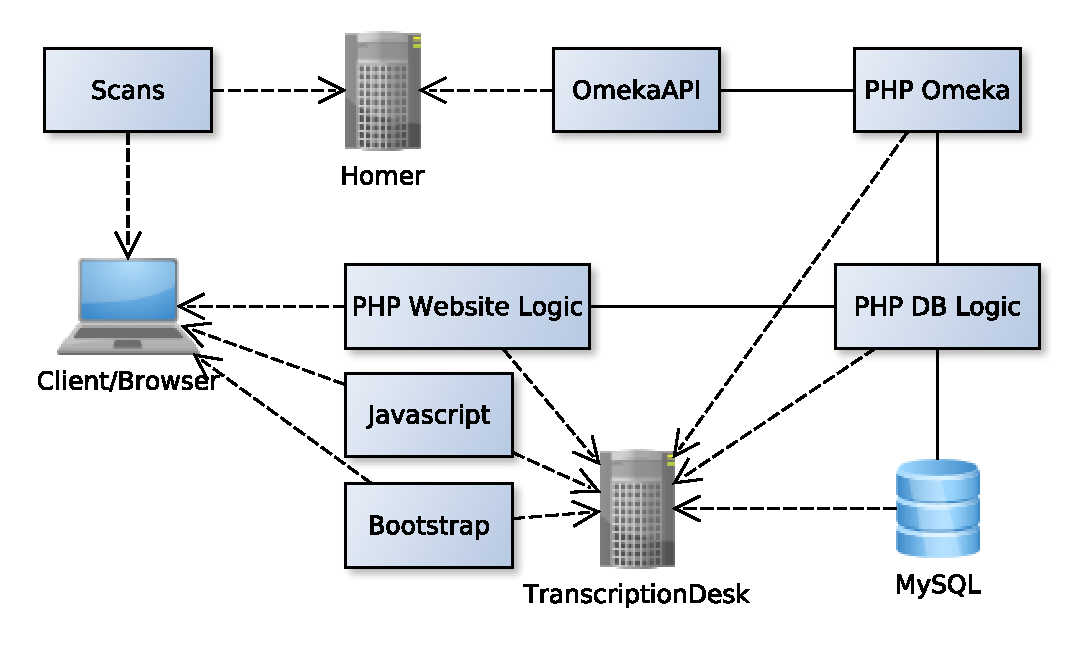
\includegraphics[width=\textwidth]{../notes/components.pdf}
\caption{Diagramm einzelner Komponenten der TranscriptionDesk Website}
\label{fig:components}
\end{figure}
Auf dem Homer Server ist eine Instanz der Omeka\footnote{\url{http://omeka.org/}} Software installiert.
Innerhalb dieser Instanz werden die Scans verwaltet und anderen Teilnehmern im Internet bereitgestellt.
Um Informationen über einzelne Scans, deren Metadaten und Sammlungen von Scans verfügbar zu machen,
stellt Omeka eine eigene API bereit, von der wir mittels der PHP Omeka Komponente in regelmäßigen Zeitabständen Daten sammeln.\\
Die auf der TranscriptionDesk-Installation laufende MySQL Datenbank dient als Speicherplatz für alle eingehenden Informationen,
sie wird gegenüber dem Rest der Website durch die PHP DB Logic Komponente gekapselt,
die aus einer Reihe von Klassen besteht, deren Aufgabe es ist,
Teile der domänenspezifischen Logik und Queries an die Datenbank zusammenzufassen
und für den Rest des PHP Codes verwendbar zu machen.\\
Aufgabe der PHP Website Logic ist es, aus den vorliegenden Informationen eine Website zusammen zu setzen
und den zu verwendenden JavaScript Code sowie von uns genutzte Teile des Bootstrap frameworks in die Website einzubetten.
Bootstrap und JavaScript sind hier als getrennte Komponenten dargestellt,
da sie sich prinzipiell auch auf andere Server verschieben lassen.\\
Zum Anzeigen von Scans auf dem Clientgerät baut der Client neben der Verbindung zum TranscriptionDesk Server auch eine Verbindung zu Omeka auf,
um die anzuzeigenden Scans zu erhalten.

\subsection{Verwendete Technologien}
In diesem Abschnitt werden die Technologien erläutert,
die zum realisieren der TranscriptionDesk Website genutzt wurden.
Als Grundlage des Entwicklungsprozesses griff die Projektgruppe auf Vagrant\footnote{
    \url{https://www.vagrantup.com/}}
zurück, welches darauf abzielt, eine einheitliche und minimale Entwicklungsumgebung zu schaffen.
Dies wird möglich, indem Vagrant eine virtuelle Maschine provisioniert\footnote{
    Es lässt sich mit Docker auch eine reine Containerlösung nutzen.\\
    \url{https://www.docker.com/}},
die einem genau festgelegten Setupscript, dem Vagrantfile, folgt.
Da dieses Setup unabhängig von der sonstigen Konfiguration der Entwicklermaschine ist,
lassen sich leicht einheitliche Ausgangsbedingungen etablieren.
Zudem ist es später leicht machbar, Vagrant zu benutzen,
um das Projekt auf einem Server einzurichten.
Bei unserem Setup gehen wir von einem Ubuntu Vivid 64bit aus,
das mit Systemd\footnote{
    \url{https://wiki.freedesktop.org/www/Software/systemd/}}
läuft. Systemd ist ein neuerer System- und Servicemanager für Linux,
den wir uns im speziellen zu nutze machen,
um mittels Timer in regelmäßigen Zeitabständen
einen PHP Script auszuführen,
der Daten von Omeka sammelt.
Innerhalb unseres Vagrantsetups betreiben wir einen LAMP-Stack\footnote{\url{https://en.wikipedia.org/wiki/LAMP_(software_bundle)}},
das heißt, dass wir die weit verbreitete Kombination von Linux, Apache2\footnote{
    \url{https://httpd.apache.org/}}, MySQL\footnote{
    \url{https://www.mysql.com/}} und PHP\footnote{
    \url{https://secure.php.net/}} nutzen.
Basierend auf dieser serverseitigen Installation liefern wir eine Website an die Browser der Nutzer aus,
die JavaScript\footnote{
    \cite{Flanagan},
    \url{https://en.wikipedia.org/wiki/JavaScript}} enthält, das es uns ermöglicht,
erweiterte Funktionalitäten im Browser bereit zu stellen,
und so komplexere Aufgaben wie das Markieren von Areas of Interest
auf einer angenehmen Oberfläche zu präsentieren.
Dabei greifen wir auf unterschiedliche JavaScript Bibliotheken zurück:
\begin{description}
\item[jQuery:]
    Bei jQuery\footnote{\url{https://jquery.com/}} handelt es sich um eine beliebte JavaScript Bibliothek,
    welche die Manipulation und das Durchsuchen des DOM\footnote{\url{https://en.wikipedia.org/wiki/Document_Object_Model}} sowie
    den Umgang mit Events und Ajax\footnote{\url{https://en.wikipedia.org/wiki/Ajax_(programming)}} Requests vereinfachen soll.
\item[Ace:]
    Ace\footnote{\url{https://ace.c9.io/}} ist ein Code Editor, der unser Projekt um die Möglichkeit anreichert,
    Markdown mit Syntax Highlighting und Zeilennummern einzugeben.
\item[OpenLayers:]
    OpenLayers\footnote{\url{http://openlayers.org/}} ist eine Bibliothek zum Umgang mit Kartenmaterial.
    Im TranscriptionDesk Projekt benutzen wir diese Bibliothek,
    um einzelne Scans, den Stücken einer Karte gleich, darzustellen,
    und das verschieben und zoomen mit selbigen zu ermöglichen.
\item[jQuery UI:]
    Bei jQuery UI\footnote{\url{https://jqueryui.com/}} handelt es sich um eine Sammlung von Hilfsfunktionen für den Umgang mit User Interfaces.
    Konkret findet es beim Ändern der Größe einiger Steuerelemente Anwendung.
\item[bootstrap:]
    Bootstrap\footnote{\url{http://getbootstrap.com/}} ist ein populäres HTML, CSS und JavaScript Framework,
    das grundlegende Elemente zur Gestaltung der Website liefert, die in allen gängigen Browsern bereits auf Kompatibilität geprüft wurden.
\item[bootbox.js:]
    Bootbox.js\footnote{\url{http://bootboxjs.com/}} ist eine kompakte JavaScript Bibliothek,
    die Bootstrap um Möglichkeiten ergänzt,
    einfach Dialogboxen zu erstellen und die Reaktionen von Nutzern auf diese zu verarbeiten.
\item[require.js:]
    Require.js\footnote{\url{http://www.requirejs.org/}} bietet ein Modulsystem für JavaScript,
    welches sich vom Browser aus benutzen lässt.
    Nebeneffekte von Require.js sind, dass sich der Code später leicht minifizieren lässt,
    und asynchron geladen werden kann.
\end{description}
\subsection{Datenbank}
In diesem Abschnitt widmen wir uns dem Aufbau der Datenbank.
Da wir mit MySQL eine relationale Datenbank einsetzen,
werden anfallende Daten auf einzelne Tabellen verteilt gespeichert,
die zueinander in Relation stehen.
\begin{figure}[H]
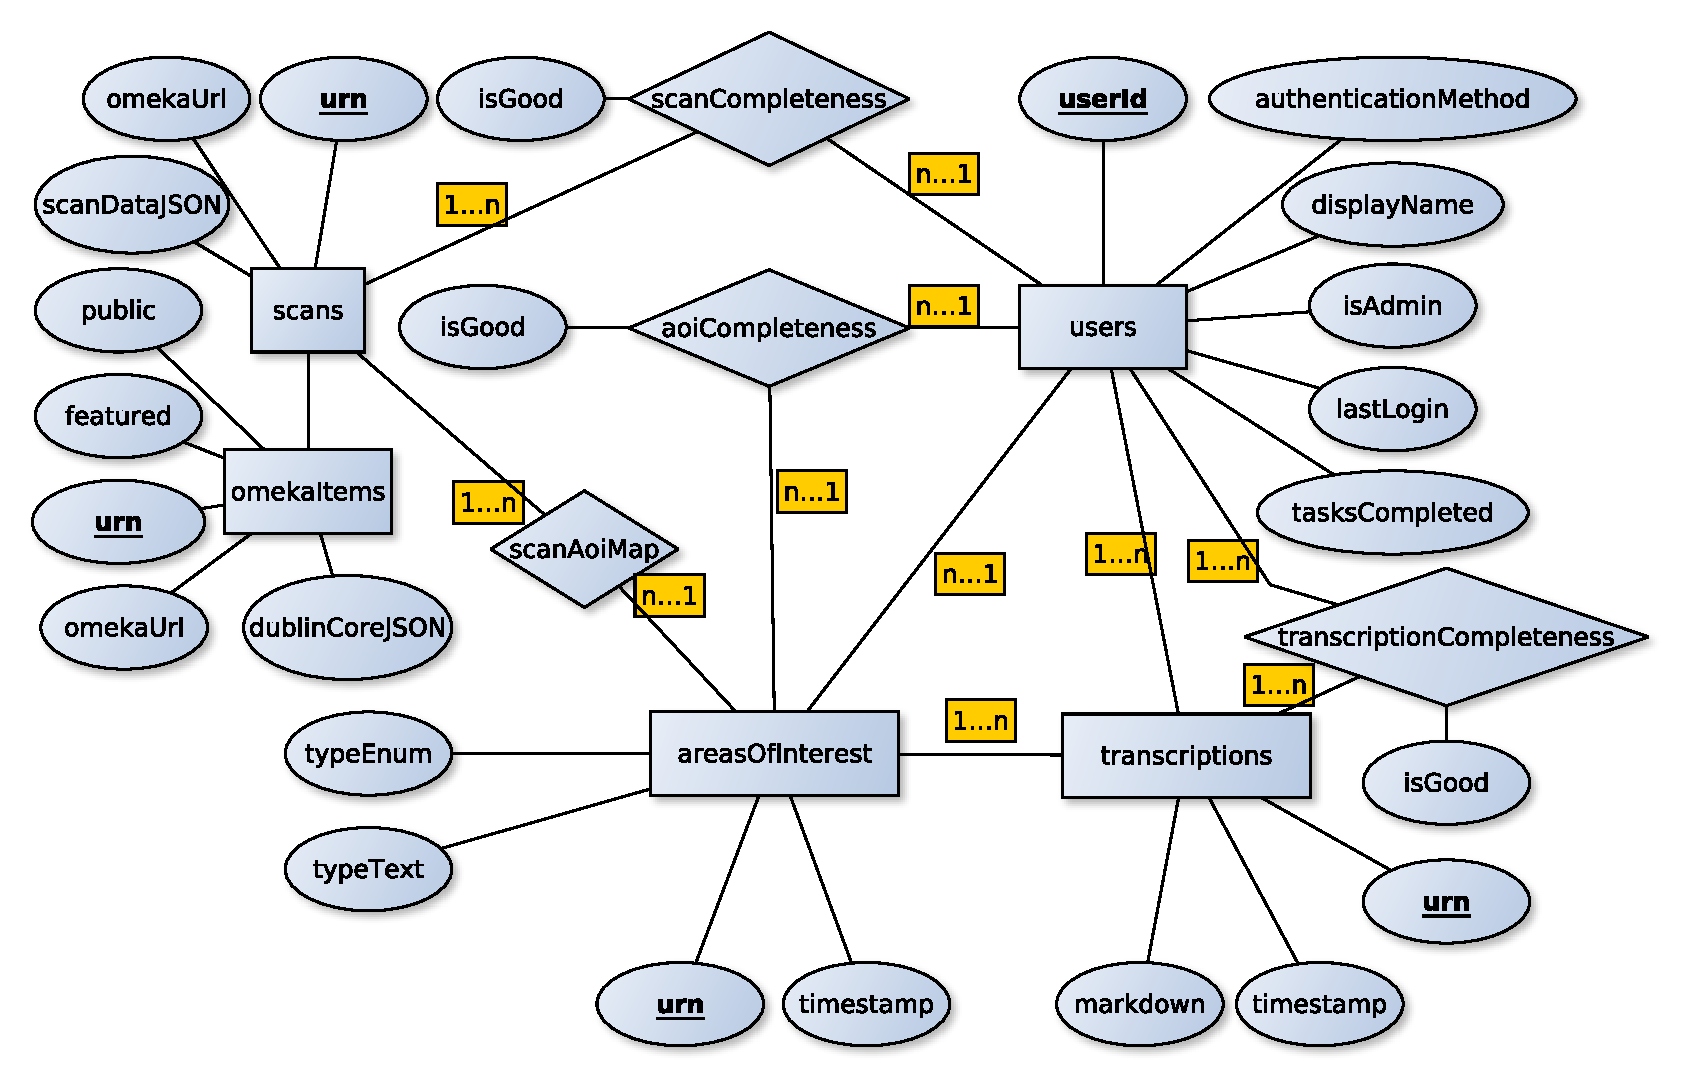
\includegraphics[width=\textwidth]{../notes/ER.pdf}
\caption{Entity-Relationship Diagramm der Datenbank}
\label{fig:er}
\end{figure}
Wie dem Entity-Relationship Diagramm in Abbildung \ref{fig:er} entnommen werden kann,
gibt es in unserer Datenbank fünf grundlegende Tabellen,
und vier weitere Tabellen,
die $n:m$ Relationen zwischen diesen realisieren.
\begin{description}
\item[omekaItems:]
    Die Tabelle omekaItems wird von einem Systemd Timer,
    der die Omekainstanz auf Homer crawlt,
    regelmäßig mit Daten befüllt.
    Um eindeutig feststellen zu können,
    welche Datensätze geändert und welche hinzugefügt werden müssen,
    speichern wir dafür sowohl die URL,
    als auch die zugehörige URN jedes Items.
    Um Aufschluss darüber zu haben,
    ob und welchen Besuchern wir bestimmte Datensätze anzeigen dürfen,
    hat jeder Datensatz Booleans in den Feldern public und featured.
    Die von diesen Feldern abgeleitete Zugriffslogik sieht wie folgt aus:

    \begin{tabular}{r|l}
    Nutzer & Bedingung\\\hline
    Unregistrierter Besucher & $\texttt{public}\land\texttt{featured}$\\
    Registrierter Benutzer & $\texttt{featured}$
    \end{tabular}

    Weiterhin gibt es noch das Feld dublinCoreJSON,
    in dem die Dublin Core Daten aus Omeka im JSON Format abgelegt werden.
    Diese Abweichung vom relationalen Paradigma bei Datenbanken wählten wir,
    da die Dublin Core Daten sich teilweise stark unterscheiden,
    und keiner gezielten Selektion durch SQL bedürfen.
\item[scans:]
    In der Tabelle scans sammeln wir die Daten zu allen einzelnen Scans,
    wie wir sie mittels des Systemd Timers erhalten.
    Genau wie die omekaItems Tabelle hat auch die scans Tabelle Felder für URN und URL.
    Zusätzlich gibt es das Feld scanDataJSON,
    in dem Metadaten zum Scan gesammelt werden.
    Dazu zählen etwa die unterschiedlichen Auflösungen,
    in denen ein Scan verfügbar ist
    oder das Dateiformat des Scans.
\item[areasOfInterest:]
    Alle von Nutzern der TranscriptionDesk Website markierten Areas of Interest werden in der areasOfInterest Tabelle gespeichert.
    Für jede Area of Interest wird eine eindeutige URN generiert,
    und der Zeitstempel ihrer Erstellung gespeichert.
    Da Areas of Interest einen Typ und in manchen Fällen auch eine Beschreibung haben sollen,
    gibt es in dieser Tabelle die Felder typeEnum und typeText.
\item[transcriptions:]
    Die transcriptions Tabelle ordnet jeder Area of Interest eine Transcription im Markdown format zu,
    sowie den Zeitstempel des Speicherns und eine eindeutige URN, die von der zugehörigen Area of Interest abgeleitet wird.
\item[users:]
    Um Nutzern die Registerierung zu ermöglichen,
    sowie eine einfache Rechteverwaltung zu etablieren,
    gibt es die Tabelle users.
    Jeder Eintrag dieser Tabelle verfügt über eine eindeutige Nummer, die userId.
    Im Feld authenticationMethod speichern wir JSON encodiert Daten,
    die den Authentikationsservice beschreiben,
    und eine eindeutige Zuordnung eines Nutzers zu einem Authentisierungsservice wie z.B. GitHub ermöglichen.
    Um Nutzern einen grundlegenden Grad von Anonymität zu ermöglichen,
    gibt es das Feld displayName,
    in dem der Name des Nutzers eingetragen ist,
    der auf der Seite angezeigt werden soll.
    Wir speichern außerdem im Feld tasksCompleted
    die Anzahl der Aufgaben, die ein Nutzer erledigt hat,
    d.h. die Summe aller erstellten Areas of Interest, Transkriptionen,
    und teilgenommener Abstimmungen.
    Um feststellen zu können, welche Area of Interest oder welche Transkription
    von welchem Nutzer erstellt wurden,
    haben die jeweiligen Tabellen Felder,
    die auf einen Eintrag in der users Tabelle verweisen.
\end{description}
Neben diesen grundlegenden Tabellen sind 3 weitere Tabellen hervorzuheben:
Die Tabellen aoiCompleteness, scanCompleteness und transcriptionCompleteness
realisieren Abstimmungen über die Vollständigkeit der jeweiligen Areas of Interest, Transkriptionen, und Scans.
Das bedeutet, dass Nutzer abstimmen können,
für wie gelungen sie eines der jeweiligen Artefakte halten,
und ob sie die Arbeit mit diesem für beendet erklären wollen.
Bei diesen Abstimmungen können Nutzer entweder zustimmen oder ablehnen.
In der Software lässt sich eine Anzahl Stimmen konfigurieren,
die für Zustimmung oder Ablehnung notwendig ist,
und als Entscheidung der Nutzerbasis gewertet wird.
Stimmt ein als Administrator markierter Nutzer ab,
so wird dessen Stimme sofort als Entscheidung gewertet.

\section{Projektverlauf}
In diesem Abschnitt möchten wir den Verlauf unseres Projektes von den ersten Treffen bis hin zum finalen Stand kurz skizzieren.
Wir möchten dabei vor allem auf Schwierigkeiten eingehen und die unterwegs aufgetretenen Probleme sowie die Designentscheidungen genauer betrachten. \\
Wir begannen das Projekt nach einer Analyse der Aufgabenstellung mit der Recherche von Technologien auf deren Basis wir bereits möglichst viele Produktfunktionen ohne Programmierarbeit abbilden konnten.
Danach planten wir die groben Entwicklungsetappen in drei Meilensteinen in GitHub nach dem Modell der agilen Softwareentwicklung wie in Punkt 3.1 beschrieben.\\
Die Planung zum ersten Meilenstein drehte sich vor allem um die Frage nach dem Datenfluss, um die Scans vom Fileserver dem Nutzer bei der Transkription zur Verfügung zu stellen, 
ohne die jeweiligen Dateirechte zu verletzten und außerdem um die Algorithmik hinter dem System der Areas of Interest, welche der im Homer Multitext entwickelten Lösung ähneln sollte. 
Wir entschieden uns für die Implementierung von Rechtecken parallel zur Seite, 
um Areas of Interest zu markieren und planten den in Kapitel 4 beschriebenen Datenfluss über den Omeka-Server.\\
In den nächsten Treffen analysierten wir die Aufgabenstellung genauer und ordneten das Projekt in die Kategorien der Citizen Science nach Haklay ein. (siehe Kapitel 2.3) 
Um das Projekt unserer Analyse entsprechend vom Crowdsourcing abzuheben, beschlossen wir ein accountbasiertes Nutzermanagement und entschieden uns dafür, die Nutzerdaten nicht selbst zu speichern,
sondern die Authentifizierungs-APIs großer Internetgemeinschaften wie z.B. Facebook, Twitter und GitHub anzubinden, so dass sich Nutzer über ihren Account auf diesen Plattformen bei uns registrieren können.
Diese Programmroutine sollte neben der Einrichtung der Omeka-API über den uns zur Verfügung gestellten Login eine der ersten umzusetzenden Funktionen sein.\\
Unser gewähltes agiles Entwicklungsmodell erlaubte es uns, diese Funktionen in kurzer Zeit arbeitsteilig zu implementieren.
Wir beschränkten uns nach kurzer Diskussion darauf, den Registrierungsprozess ausschließlich über die GitHub-API laufen zu lassen, zusätzliche Authentifizierungsscripte nur in den Programmquellen zu hinterlegen und in der Oberfläche auszublenden. 
Der Grund dafür war insbesondere der umfangreiche Registrierungsprozess einer Applikation bei Facebook, welches unter anderem eine Rechteaufgabe an der Software beinhaltet.\\
Die verschiedenen Lizenzen und Dateirechte der Scans abstrahierten wir im Wesentlichen zu den zwei Klassen ,,public'' und ,, featured'', während letztere nur eingeloggten Nutzern sichtbar sind.(siehe Kapitel 5.3.)\\
Der nächste Schritt war die Planung und der schrittweise Aufbau des Datenbankmodells wie in Kapitel 4.3 beschrieben. 
Außerdem entschieden wir uns für Docker als vereinheitlichende Plattform für die gemeinsame Entwicklung mit gleichen Systemvoraussetzungen.
Die Einrichtung von Docker bereitete uns insbesondere auf Windows-Umgebungen Probleme.\\
Im weiteren Verlauf der Arbeit am ersten Meilenstein diskutierten wir über das Votingsystem zur Validierung der Areas of Interest und Transkriptionen und 
erweiterten das Datenbankschema entsprechend. 
Dieses System soll auch dem Missbrauch der Plattform durch Speicherung offensichtlich falscher Transkriptionen vorbeugen.\\
In den folgenden Projektwochen konnten die Probleme mit Docker in der Virtualbox nicht gelöst werden, worauf wir nach kurzer Recherche mit einem Umstieg auf Vagrant reagierten.
Dieses sollte sich gerade unter Windows einfacher einrichten lassen und somit das Projekt kaum verzögern.
Parallel dazu wurde von Herrn Koentges gefordert, alle finalen Transkriptionen im Markdown-Format automatisiert auf GitHub zu speichern und
die in den Scans verwendeten handschriftlichen Sondersymbole durch ein MUFI-Eingabesystem in utf-8 abzuspeichern.
Diese Ideen übernahmen wir in den Anforderungskatalog und fügten sie agil dem zweiten Meilenstein hinzu.\\
In dieser Zeit schlossen wir auch den ersten Meilenstein mit einem Prototypen der Plattform ab. 
Mit diesem war es bereits möglich, sich über GitHub als Nutzer zu registrieren, eine Demo von OpenLayers zu betrachten und 
auf einer Grafik Areas of Interest zu markieren, die jedoch noch nicht gespeichert wurden. 
Zusätzlich dazu war im Hintergrund schon die Verbindung zu Omeka eingerichtet und es war möglich, 
Daten zu crawlen und in einer Liste zusammenzufassen. Der gesamte Prototyp lief in einem Vagrant Container.\\
Direkt im Anschluss daran begannen wir mit der Arbeit am zweiten Meilenstein. 
Dieser umfasste hauptsächlich die Umsetzung einer Eingabemaske für Mufi-Symbole, die Programmierung des Votingsystems für die Areas of Interest sowie die Umsetzung des Datenflusses mithilfe von OpenLayers.
In diesem Zusammenhang bekamen wir noch die Anforderung, die Areas of Interest in Kategorien zu sortieren. Diese sollten ,,Main Text'', ,,Marginal Text'', ,,Image'', ,,Mathematical Figure'', ,,Other (Freetext description)'', ,,Initials'' und ,,Title'' 
umfassen und gemeinsam mit den Identifikatoren des Rechteckes gespeichert werden.
Wir passten das Datenbankschema entsprechend an und fügten diese Anforderung dem dritten Meilenstein hinzu.\\
Für die Umsetzung des Mufi-Eingabesystems planten wir, ein virtuelles Keyboard an die Eingabemaske anzuhängen, 
mit dessen Hilfe dynamisch utf8-Symbole in das Markdown-Eingabefeld geparst werden könnten 
um anschließend live den Markdown Code zu rendern.
Eine Vorlage für ein solches Keyboard fanden wir mit dem Mottie Virtual Keyboard\footnote{\url{https://mottie.github.io/Keyboard/}}.
Erst nach der Aufbereitung der Zeichentabelle und dem Hinzufügen der Programmquellen für das Keyboard fanden wir die Anzeige von weit mehr als 500 Symbolen\footnote{Vergleiche MUFI Character Database\\\url{http://www.abdn.ac.uk/skaldic/db.php?if=mufi&range=AlphPresForm&table=mufi_char}} auf einem virtuellen Keyboard sehr unpraktisch und 
entschieden uns daher für die Implementierung einer Tag-Suche auf Kategorien von Symbolen, so dass das gewünschte Symbol wesentlich leichter für Nutzer zu finden ist.\\
Mit dem Ende der Vorlesungszeit intensivierten wir die Implementierungsarbeiten am Projekt und konnten schnell weitere Teile des zweiten Meilensteins abschließen. 
In dieser Phase des Projektes bereitete uns der Vagrant Container unerwartete Probleme. 
Aufgrund eines Defekts musste ein neuer Laptop eingerichtet werden, welcher in der Konfigurationsebene des BIOS zunächst keine Virtualisierung unterstütze.
Aus diesem Grund verzögerte sich die Entwicklung von OpenLayers und überschnitt sich zeitlich mit dem dritten Meilenstein, 
was besondere organisatorische Fähigkeiten erforderte.
Die Organisation des Projektes mit Hilfe von sog. ,,Issues'' im GitHub half uns, den Überblick im Team zu bewahren.\\
Zu den Issues des dritten Meilensteins gehörte die Verbesserung der Profilseite und das Handling der Transkriptionen.
Dies beinhaltet das Votingsystem, sowie die Speicherung und die Veröffentlichung der von den Nutzern als gut bewerteten Transkriptionen auf GitHub.\\
An diesen Issues arbeiteten wir bis zum Ende des Sommersemesters und beendeten die Arbeit am Projekt mit einer Liste an offenen Issues,
die unter \url{https://github.com/runjak/TranscriptionDesk/issues} eingesehen werden können.

\section{Zusammenfassung und Ausblick}
Insbesondere die Organisationsform über GitHub und das Issue-System sind Dinge, welche wir positiv aus dem Projekt für zukünftige Arbeiten mitnehmen.\\
Wir kennen aus der Informatik die Theorie der agilen Entwicklungsmodelle sowie ihre Stärken und Schwächen, weshalb es für uns immer wieder spannend ist, diese im praktischen Einsatz zu erleben.
Aufgrund dieser Möglichkeiten und unseren Vorkenntnissen im Bereich der Webentwicklung fiel unsere Wahl auf das TranskriptionDesk Projekt.
Zwar besaßen wir kaum fachliche Vorkenntnisse in Bezug auf die Datenbasis und beherrschen die lateinische Sprache nicht, doch an dieser Stelle konnte uns Herr Koentges das notwendige Fachwissen und entsprechende Dokumentation vermitteln.\\
Unser Projektteam selbst war sehr gemischt und deckte verschiedenste Bereiche der Informatik ab. So bildeten wir ein Team aus Masterstudenten 
spezialisiert auf einerseits Softwaretechnik und Semantic Web und andererseits Web- und Anwendungsentwicklung sowie Management und Datenbankadministration.
Als besonders wichtig erachten wir deswegen in der nachträglichen Betrachtung die Verwendung einer einheitlichen Entwicklungsumgebung in der gesamten Gruppe. 
Wir hätten mehr Zeit für die Recherche von Vagrant und dem Vergleich zu Docker verwenden müssen, um den Problemen und Verzögerungen vorzubeugen.\\
Nur durch die Erfahrungen, welche wir aus dem Projektmanagement und der Softwaretechnik mitbrachten war es uns möglich, diese Schwierigkeiten direkt anzugehen und dynamisch auf neue Anforderungen zu reagieren.
Das ermöglichte uns, in agiler Planung ausreichend Zeit für Zwischenrecherchen (MUFI-System, OpenLayers, usw.) einzuräumen und eine effiziente Software fertigzustellen.
Mit dem Fokus auf Modularisierung, Wiederverwendung und Wartbarkeit sollten sich die administrativen Aufgaben in einem moderaten Rahmen bewegen und 
durch das Verfolgen eines strikten Open-Source Paradigmas in der Entwicklung können unsere Erfahrungen zukünftigen Teams dabei helfen, ähnliche Projekte zu realiseren.
Wir hoffen, dass unsere Software den Weg in den Produktiveinsatz finden wird, was laut den Webquellen des Lehrstuhls für Digital Humanities an der Uni Leipzig bereits geplant ist und bereits jetzt als eines der größten Projekte im Bereich der Transkription geschätzt wird.

\section*{Quellen}
  \printbibliography[%
    heading=bibintoc, % (bibintoc, bibnumbered)
  ]
\end{document}
